\chapter{Exercise 4}
The purpose of this exercise is to get acquainted with lighting and
shading in OpenGL and GLSL.
You will calculate the shading of an object based on the ambient,
diffuse and specular properties of the material and the light source.

\section{Part 1}
I successfully modified the vertex shader to implement Phong ligthing using Gouraud
which can be seen in figure \ref{fig:exercise_4_part_1}
\begin{figure}[ht!]
	\begin{center}
		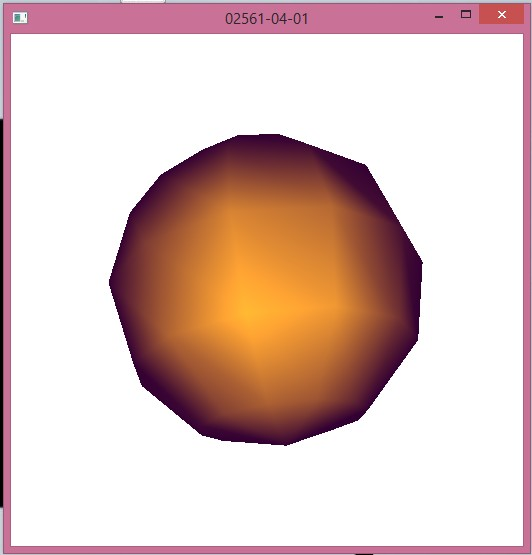
\includegraphics[width=0.5\textwidth]{figures/exercise_4_part_1}
	\end{center}
	\vspace{-4.5ex}\caption{Exercise 4 part 1 output}
	\label{fig:exercise_4_part_1} 
\end{figure}

\section{Part 2}
In the pictures below 
(figures \ref{exercise_4_part_2-1} and \ref{exercise_4_part_2-2}) 
you can see implemented
Phong shading using fragment shader also with specular contribution.
\begin{figure}[ht!]
	\begin{center}
		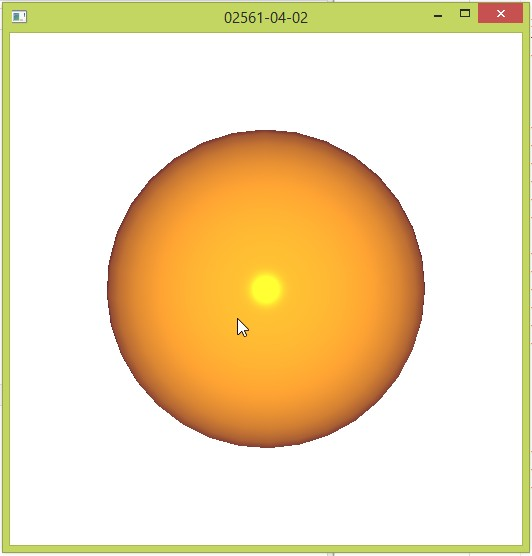
\includegraphics[width=0.6\textwidth]{figures/exercise_4_part_2-1}
	\end{center}
	\vspace{-4.5ex}\caption{Exercise 3 part 2 output (directional)}
	\label{fig:exercise_4_part_2-1} 
\end{figure}
\begin{figure}[ht!]
	\begin{center}
		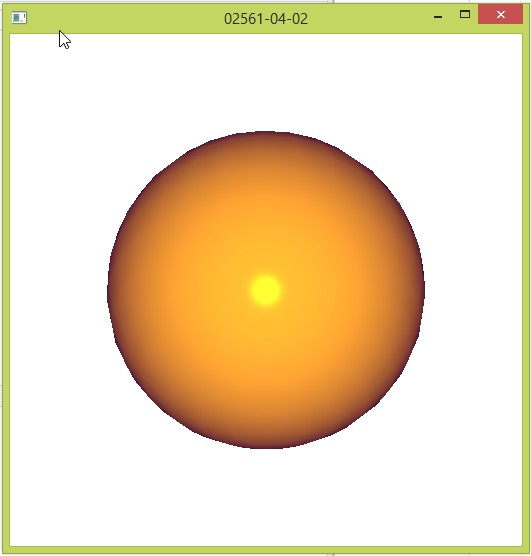
\includegraphics[width=0.6\textwidth]{figures/exercise_4_part_2-2}
	\end{center}
	\vspace{-4.5ex}\caption{Exercise 4 part 2 output (point)}
	\label{fig:exercise_4_part_2-2} 
\end{figure}
\clearpage

\section{Part 3}
\begin{description}
\item[Phong shading and Phong lighting]
	Phong lightning is a model of lightning where object surface is covered by thin transparent layer,
	where specular reflection takes place. While Phong shading is a technique of shading the polygons,
	where a normal vector is interpolated between vertices and then any lightning model is used for 
	interpolated pixels. 
\item[Gouraud shading and Phong shading]
	This two shading methods differs how a normal vector is assigned to pixels when calculating a color.
	In Goroaud shading color is calculated for every vertex using its normal vector, and then color is
	interpolated, while in Phong shading normal vector is interpolated and color is calculated for each pixel.
	Goraud shading is faster but less accurate than Phong shading.
\item[Point light and directional light]
	In directional light, rays are parallel to each other.
\item[Eye position any influence]
	Eye position is substantial in rendering reflections of the light from shiny objects.
\item[Specular term equal to $(0,0,0)$]
	The reflection disappeares.
\item[Increasing shininess exponent]
	When shininess exponent is inceased the reflection is getting smaller and it is more simillar to a perfect mirror.
\item[Simplifications] No simplifications were used.
	
\item[Normal matrix]
	Normal matrix is used to transform the normal into eye space. We only want to transform its orientation. 
	The region of the modelview matrix that contains the orientation is the top left $3*3$ submatrix. The reason
	of using normalized matrix is that a modelview matrix can contain a non-uniform scale. Because of that we
	compute this matrix as:
	\begin{lstlisting}[language=cpp, caption={Normal matrix}]
	normalize(transpose(inverse(mat3(ModelView))) * fragNormal);
	\end{lstlisting}
\item[Light coordinate space]
	I use eye space coordinate system because it is easier to calculate specular light effect.
\end{description}
\clearpage

\section{Part 4}
I implemented Phong shading for multiple light sources with different colors and attributes.
It is done using code below in the fragment shader and the results can be seen in the figure
\ref{fig:exercise_4_part_4}

\begin{figure}[ht!]
	\begin{center}
		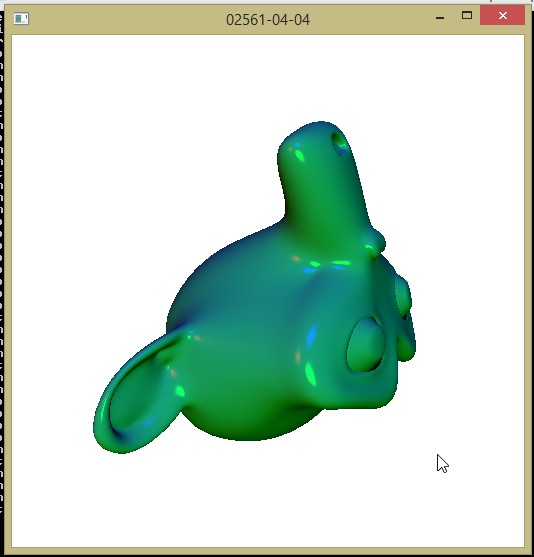
\includegraphics[width=0.75\textwidth]{figures/exercise_4_part_4}
	\end{center}
	\vspace{-4.5ex}\caption{Exercise 4 part 4 output}
	\label{fig:exercise_4_part_4} 
\end{figure}

\begin{lstlisting}[language=cpp, caption={Phong lightning}]
uniform mat4 ModelView;
uniform vec4 MaterialColor;
uniform vec4 MaterialSpecularColor;
uniform float Shininess;
#define MAX_LIGHTS 5
uniform int NumLights;
uniform struct Light {
	vec3 position;
	vec3 color;
	float lightType;
	float attenuation;
	float ambientCoefficient;
} Lights[MAX_LIGHTS];
in vec3 fragPosition;
in vec3 fragNormal;
out vec4 fragColor;

vec3 ApplyLight(Light light, vec3 normal, vec3 position)
{
	vec3 surfToLight = normalize(light.position);
	float attenuation = 1.0;
	if(light.lightType == 1.0)
	{
		surfToLight = normalize(light.position - position);
		float distance = length(light.position - position);
		attenuation = 1.0 / (1.0 + light.attenuation * pow(distance, 2));
	}
	vec3 surfToCamera = normalize(position);
	vec3 reflection = reflect(surfToLight, normal);
	vec3 ambient = light.ambientCoefficient * MaterialColor.xyz * light.color;
	float diffuseCoefficient = clamp(max(dot(normal, surfToLight), 0.0), 0.0, 1.0);
	vec3 diffuse = diffuseCoefficient * MaterialColor.xyz * light.color;
	float specularCoefficient = diffuseCoefficient > 0 ? clamp(pow(max(dot(reflection, surfToCamera), 0.0), Shininess), 0.0, 1.0) : 0.0;
	vec3 specular = specularCoefficient * MaterialSpecularColor.xyz * light.color;
	return ambient + attenuation*(diffuse + specular);
}

void main() 
{ 
	vec3 normal = normalize(transpose(inverse(mat3(ModelView))) * fragNormal);
	vec3 position = vec3(ModelView * vec4(fragPosition, 1.0));
	vec3 linearColor = vec3(0);
	for(int i = 0; i < NumLights; ++i)
		linearColor += ApplyLight(Lights[i], normal, position);
	fragColor = vec4(linearColor, 1.0);
} 
\end{lstlisting}

